\titleformat
	{\chapter} % command
	[display] % shape
	{\bfseries\Large} % format
	{
		\vspace{-1cm}
		%Story No. \ \thechapter
	} % label
	{0cm} % sep
	{
		\vspace{-2cm}
		\begin{center}
		{
\includegraphics[width=\the\textwidth]{./Images/Chapter_Banner.png}\\
		\vspace{1.5cm}}
%		\color{red}
	} % before-code
	[
		\small\vspace*{.5cm}
			An answer to a letter received from a Russian Orthodox woman abroad, married to a Protestant, on the occasion of Count Leo Tolstoy's excommunication.\footnote{From the periodical \textit{Edifying Readings}, Moscow, No. 3, 1901.}
		\end{center}
	] % after-code

\addcontentsline{toc}{chapter}{APPENDIX B\\May Orthodox Christians Pray For Non-Orthodox Christians, And If So, How May They Pray For Them?}
\chapter*{May Orthodox Christians Pray For Non-Orthodox Christians, And If So, How May They Pray For Them?\markboth{Appendix B}{}}
\chformat

\hugered{A}LL OF US who are children of the One, Holy, Catholic, Apostolic, Ecumenical Church ought not to be guided by our own reasonings in questions which arise concerning the doctrine of our Faith, since these reasonings may be erroneous. Rather, in such instances we must apply the canons which give us guidance. These canons are contained primarily in a book called \textit{The Rudder}. This is a collection of the canons of the holy Apostles, the holy Ecumenical and Local Councils and those of several of the holy Fathers.

At the end of this book, in the chapter, “Concerning the Apostasy of Rome--how she fell away from the Orthodox Faith and from the Holy Eastern Church,” the Pope of Rome together with his followers, who wrongly call themselves catholics, are termed heretics. Concerning the other Protestant Christian confessions there is nothing to be said, inasmuch as they have departed even further from Orthodoxy.\trans{The section referred to here is not included in the Greek edition of the \textit{Rudder} (or in the English translation, which was made from the Greek edition). It is evident that it was included in the Russian edition because of the widespread efforts of the \textit{Unia} in the western regions of Russia and the Ukraine.}

In the same book, \textit{The Rudder}, in the tenth chapter, in the sixth canon of the local Council of Laodicea, the Holy Church pronounces this judgment on heretics in general: “Heretics should not be allowed to enter the House of God, so long as they persist in their heresy.” And in the thirty-third canon of the same Council of Laodicea it is stated: “It is not permitted to pray with heretics and schismatics,” that is, those who are separated from the Catholic Church.

But here we have a question: What is the view of the holy Fathers of our Orthodox Church concerning heresy? In the \textit{Patericon} of Bishop Ignaty Brianchaninov it is related concerning the righteous Agathon that certain brethren visited him on one occasion and wished to test his humility and patience. They upbraided him for being proud, a slanderer, and for leading a depraved life. The Elder acknowledged all these faults in himself and begged his visitors with tears to pray for him. When they called him a heretic, however, the Elder said that he was in no way a heretic. When the brethren asked him why the accusation of heresy alarmed him, he replied: “Because heresy is estrangement from God. The heretic is separated from the living and true God and is a communicant with the devil and his angels. He that is separated from Christ (i.e., through the false teaching concerning Christ which he confesses) no longer has God, Whom he could entreat concerning his sins, and in all respects he has perished.”\trans{This important distinction--between sin and heresy--is found throughout all patristic literature. Sin is a \textit{transgression} of the Gospel's teachings. Heresy is an \textit{alteration} of those teachings.}

And if this were not so, that is, if heresies or false teachings as the results of free thinking did not have such a pernicious significance in the Holy Church of Christ, then the holy Apostle Paul would not have written the first Christians such warnings: “Brethren, beware lest any man spoil you through philosophy and vain deceit, according to the tradition of men, according to the rudiments of the world, and not according to Christ” (Col. 2:8). And again, “There be some that trouble you, desiring to pervert the gospel of Christ. But though we, or an angel from heaven, preach any other gospel unto you than that which we have preached unto you, let him be anathema” (Gal. 1:7-8).

However, our Orthodox Church, in accordance with the love for man which characterizes her, permits prayer for those who have cut themselves off from her, that is, for heretics, as can be seen in the same book, \textit{The Rudder}, in Chapter 15, canon 66 of the local Council of Carthage.\trans{In connection with this, canon 75 of the same Council also addresses this question.} \textit{But prayers in what regard? Prayers that they leave their delusion and come to the knowledge of the truth.}

And in another book, \textit{The Orthodox Confession of the Catholic and Apostolic Eastern Church}, in the first part of the book at the end of the answer to the ninety-second question, it is also permitted to pray "for heretics and schismatics, that they be converted to the Orthodox Faith before the end of their lives.”

Thus does the Orthodox Church act. For example, in the Prayers for Commemoration of the Living and the Dead (at the end of the \textit{Horologion Psalter}) we pray, “Illumine with the light of Thy knowledge apostates from the Orthodox Faith, and those blinded by pernicious heresies, and unite them to Thy Holy, Apostolic, Catholic Church.”

Now we shall bring forth several of our own considerations. From the quotations cited above it is clear that our Orthodox Church allows prayer for heretics only while they are yet alive, and not for those who have died, and that this prayer is only for their conversion to the Orthodox Faith. When, however, we may add, a heretic, by the prayers of the Holy Church, is converted to the Orthodox Faith, then the prayer which the Church makes for him takes on a completely different form, that is, it is \textit{for the salvation of his soul}.

But how does a person achieve salvation? One of the chief conditions for the attainment to salvation is repentance. We see examples of this in the holy Gospel. The publican was justified by means of repentance (Luke 18:10-14). The prodigal son returned to the Father through repentance (Luke 15:11-32). The wise thief who was crucified with the Lord Jesus Christ entered Paradise, likewise through repentance (Luke 23:40-43). Furthermore, the Lord said concerning Himself that He came to earth in order to call sinners to repentance (Matt. 9:13). All people are in need of repentance. “For all have sinned,” as the Apostle says, “and are bereft of the glory of God” (Rom. 3:23). But even if the non-Orthodox or heretic were to desire to offer repentance before an Orthodox priest, his repentance for his sins would be ineffective. We read in \textit{The Orthodox Confession}, in Part 1, Question 113: “What must we observe in the mystery of repentance? Answer: First of all, we must observe that the penitent is a Christian of the Orthodox and Catholic Faith, for \textit{repentance without the True Faith is not repentance and is not received by God.}”

But all of this is spoken concerning living Christians who believe incorrectly or concerning heretics. What may be said concerning the souls which have departed from this life?

Although in the \textit{Extended Christian Catechism of the Orthodox Catholic Eastern Church}, in the eleventh article, it is stated that prayers offered for the souls of the dead are able to help them to attain to the blessed resurrection, especially when these prayers are united to the offering of the Unbloody Sacrifice of the Body and Blood of Christ, yet this is said concerning the souls of Orthodox Christians, and furthermore, of those who have reposed in faith. How can there be hope of salvation for the soul of one who, while believing wrongly, died in his errors without offering sincere repentance for them before the Lord? And how and for what should one pray as regards such a soul? To pray for his salvation (“With the saints grant rest”) is impossible, because in his life the heterodox did not renounce his errors and did not offer sincere repentance for them before the Lord. It is already too late to pray for the soul's turning to repentance, because the soul after its departure from the body cannot repent, since the future life is not a time for repentance but for recompense.

Furthermore, one should consider: Why should the Orthodox Church compose special “Rites” for the uniting of Roman Catholics and Protestants to the Orthodox Faith, if even without this one could pray for the salvation of their souls? However, our Holy Church unfailingly requires of every heterodox person desiring to be in communion with her that he publicly, before the entire Church, renounce his errors and receive pure Christian doctrine. Moreover, if it were possible to offer prayers in church for the salvation of the souls of heterodox who have reposed or at least for the alleviation of their lot beyond the grave, then without fail the Orthodox Church in her divine services would employ special litanies or petitions for them. However, there is no such thing in any of our church services. On the contrary, on the First Sunday of the Great Fast, in celebrating the Triumph of Orthodoxy, our Holy Church pronounces anathema, that is, separation from unity with herself, on all heretics and apostates from Orthodoxy, which would include the Latins or Roman Catholics and Protestants. How then, we ask, would the Church at one and the same time anathematize and pray for them?

In confirmation of what has been said, we here bring forth the words of our ever-memorable hierarch, the reposed Metropolitan Philaret of Moscow. He says: “It is one thing to pray that non-Orthodox churches be united to the Orthodox Church in a broad structure of prayers, which embrace the whole world, and it is another to commemorate non-Orthodox in the diptychs (the synodicons of books of commemoration) during the Mystery of the Eucharist. The heterodox, by their very heterodoxy, have separated themselves from the communion of the Mysteries of the Orthodox Church. In consequence of this, they are not commemorated during the Mystery of the Eucharist and are \textit{excluded from the diptychs}.\footnote{\textit{Notes concerning the life and era of the Hierarch Philaret, Metr. of Moscow}, by N. V. Sushkov, 1868, Suppl. p. 162.}

We note here that the words "excluded from the diptychs” lead us to conclude that the names of non-Orthodox Christians ought not to be commemorated at all in any Orthodox church service. For truly, how can they be commemorated when they are excluded from the diptychs?

One may object: That is a very strict judgment to pass. But what are we to do? We cannot, after all, force the Lord to mercy with prayer. For our God is “a jealous God” (Exod. 20:5); “Righteous is the Lord, and He hath loved righteousness” (Ps. 10:7). There have been occasions when He Himself forbade prayer for certain people. Thus, He said to the Prophet Jeremias concerning his people: “Pray not for these people, neither entreat that they be shown mercy, and do not pray or approach Me concerning them, for I shall not hear thee” (Jer. 7:16). This command of the Lord pertains to people yet alive and who, consequently, are still able to repent. But the prophet did not dare to disobey the word of the Lord, nor justify his prayer for them as a sign of love for mankind.

However, in speaking of this, we here have in mind only public prayers made in Church for the non-Orthodox, which, if the Orthodox Church were in fact to allow, she would inevitably cause very great harm and an abyss of evil to Orthodoxy. Let us think for example: Are many Orthodox Christians firm in the faith which they confess? Do not the greater portion of them have something of a weak faith, like a tiny spark which might be extinguished at any moment? And if such people were to hear in Orthodox churches the commemoration for the health or repose of Roman Catholics and Protestants, would they not quickly come to the conclusion that it must be that \textit{it is all the same no matter what you believe?} And by this there would be even more and more frequent apostasy from the Orthodox Church, if not formally, then at least in spirit. And this would be the greatest woe. The person thus led astray would not even notice that he is Orthodox in name only, while in fact he does not believe correctly, or even does not believe at all.

Likewise, the Christians of other confessions, seeing that the Orthodox Church prays for them, must of necessity come to the same conclusion concerning the equality of all faiths. This may even dissuade from union with the Orthodox Church the heterodox who would desire this. They will say, “After all, the Orthodox pray for us, even without this.”

Yet, there are some who make a stir about this, saying that all people, no matter what faith they confess, will be saved, and that the Lord did not show us which faith we ought to confess. These are the false reveries of men. That not all will be saved is evident from the holy Gospel. In depicting the Dread Judgment the Lord decisively divides all people into two camps and places some on His right, and leads them into the Kingdom of Heaven, the others on His left, and sends them “into the eternal fire, prepared for the devil and his angels” (Matt. 25:31-46). And those who inherit the Kingdom of Heaven will be the smaller part; even from among the Orthodox it will be only those who live in an Orthodox manner. This is also evident from the words of the Lord Himself: “Many are called, but few are chosen” (Matt. 20:16). Concerning the second statement, that is, that the Lord has not shown us which faith we ought to confess, we must say that this is slander against God. For is it not for this cause that the Son of God came to earth, in order to teach people a clear and exact doctrine concerning how they ought to believe, and to arrange their life according to that faith? Therefore He said: “Think not that I am come to destroy the law” of Moses, “but to fulfil” it (Matt. 5:17). And furthermore, He spoke concerning Himself: ``I am the way, the truth and the life'' (John 14:6). And His teaching is called ``the words of eternal life'' (John 6:68). Therefore, He called all to Himself, saying ``If any man thirst, let him come unto Me, and drink'' (John 7:37). And again, ``Come unto Me all ye that labour and are heavy laden,'' and the rest (Matt. 11:28, 29). And after the Resurrection, in sending His disciples to preach, the Lord commanded them to teach all nations to observe all that was commanded by Him (Matt. 28:20). The Apostles set forth in writing in the holy Gospel and in their Epistles all that was commanded by the Lord, the true doctrine concerning the faith and how one ought to live. The holy Fathers and the teachers of the Church of Christ who came after them explained in detail all this doctrine concerning the faith and how one ought to live, as contained in the Holy Scripture, in all fullness and purity, without any admixture of incorrect human opinions and reasonings. And in the beginning, the Church of Christ was one and the same throughout the entire world. Only from the ninth century on did the Popes of Rome of their own self-will begin to add to the true teaching of Christ their own false reasoning from which the Roman Church became separated from the Orthodox Eastern Church. And te more time progressed, the more were errors added in the Roman Church until finally certain Roman Catholics dissatisfied with her fell away from her and formed their own Protestant churches which departed even further from Orthodoxy.

Concerning the importance of obedience to the Church of Christ, the Lord Himself said in the holy Gospel: ``if anyone refuse to hear the church, let him be unto thee as the heathen man and the publican'' (cf. Matt. 18:17).

Let us, however, return to our main topic. What is the significance of the fact that the Orthodox Christians do not ask Roman Catholics and Protestants to pray for them and for their deceased? On the contrary, it is the latter who not infrequently ask the Orthodox to serve \textit{pannikihidas} for their relatives, etc. What is the reason for this? Evidently, it is the poverty of the inner spiritual content of the Western heterodox Christian churches. The soul of the Roman Catholic or Protestant, thirsting for salvation, cannot find in his own church satisfaction for his highest spiritual needs. Therefore he turns to the Orthodox Church, to which alone belongs ``all the power of the Divinity which is unto life and godliness'' (cf. II Peter 1:3).

This is confirmed in very deed. Not infrequently, heterodox who have sincerely united themselves to the Orthodox Church, soon after their union and communion of the Divine Mysteries of the Body and Blood of Christ, fell in their souls an inexplicable spiritual consolation of which formerly, prior to their union to the Orthodox Church, they had no understanding. Something which can further serve as proof of the impoverishment of the Western churches is the fact that their defenders always assert their false rationalities with passion and bitterness against our Holy Orthodox Church. But in Holy Scripture it is said concerning God, ``In peace is His dwelling'' (Ps. 75:3). This means that where there is peace and love there only is there God. Where there is bitterness and lack of peace, however, there the grace of God cannot be, and the Lord does not take pleasure in embittered hearts.

However, in speaking of the strictness of our Orthodox Church concerning the commemoration of Christians who believe incorrectly, we do not mean to say that our Holy Churchcommands us, her children, not to pray for them in any way at all. She only prohibits us to pray in a self-willed fashion, that is, praying as we wish and in whatever manner might come into our heads. Our Mother the Orthodox Church teaches us that everything we do, even prayer itself, should be done ``properly and according to order'' (I Cor. 14:40). And we do pray in all our church services for all nations of diverse peoples and for the whole world, more often than not without our knowing and understanding this. We pray exactly as our Lord Jesus Christ taught His Apostles to pray in the prayer He taught them, ``Thy will be done on earth as it is in Heaven!'' This all-embracing petition gathers within itself all our needs and the needs of all our brothers, even though they be non-Orthodox. In it we entreat the All-good Lord even for the souls of the departed non-Orthodox Christians, that He may accomplish with them that which is pleasing to His holy will. For the Lord knows immeasurably better than we to whom to show mercy and what mercy to show. And thus, Orthodox Christian, whoever you may be, layman or priest of God, if during some church services there comes upon you the zeal to pray for some Carl or Edward who is close to you, then during the Lord's Prayer, sigh to the Lord on his behalf and say, ``May Thy holy will be done in him, O Lord!'' and limit yourself to this prayer. For thus have you been taught to pray by the Lord Himself. And believe that this prayer of yours made in such a way ill be a thousand times more pleasing to the Lord and more profitable to your soul than all your self-willed commemorations in church.

All of the thoughts which we have expressed above, and which are, as anyone can see, founded on Sacred Scripture and the Tradition of the holy Fathers, naturally lead to the conclusion that to pray with the common prayers of the church for Orthodox Christians and for non-Orthodox Christians on an equal basis, that is, to commemorate their names in church in the same way as the names of Orthodox Christians are commemorated, is not in accord with the teaching and ordinaces of our One, Holy, Catholic, Apostolic, Ecumenical Church. Thus do we speak, and thus do we act. And this not at all out of hatred toward those Christians who believe wrongly, nor because we do not wish them well but because our self-composed or self-willed prayer for them will not be pleasing to God, will be without benefit for their souls, and will be accounted as sin for those who pray thus for them. A clear example of this may be seen in the life of Saul, the king of Israel. He had to all appearances done a good deed when he turned to God with prayers and offerings of sacrifices before beginning his war with the Philistines. But inasmuch as he acted in this case on his own will, without waiting for Samuel the prophet of God, as had been commanded him, he not only did not draw to himself the good pleasure and blessing of God, but even earned God's wrath and punishment. Let us add here that self-will in every matter is a sin and even among men an intolerable fault. There has come about the saying, ``Let the Tsar be sick that your own will may prevail.'' Yet, we see that the Tsar punishes those who do not submit to the imperial laws. Why? Because he who does his own will causes harm to himself, to his family, and to the society in which he lives, as well as to the government and the Church. In a word, the man who does his own will is an unacceptable person. Those who do their own will do not themselves like those who do not submit to them, and if they have the opportunity they punish them. But we all want to live and pray, each one as he sees fit.

Now let us say a few words about private prayer. In our Orthodox Church there is scarcely more than one example of how the private prayer of a saint of God aided the souls of deceased heterodox, even of pagans. Saint Macarius of Egypt tells the following concerning himself: ``Once, while going through the desert, I found the skull of a certain dead man lying on the ground. When I struck the skull with my palm staff, it spake to me. I asked it, 'Who are thou?' The skull answered me, 'I was the chief priest of the idols and the pagans who dwelt in this place, and thou art Macarius the Spirit-bearer. When thou takest pity upon those suffering in torment and beginnest to pray for them, they feel a certain consolation.' The Elder asked him 'What is the consolation, and what the torments?' The skull said to him 'As far as the heaven is above the earth, so much is there fire beneath us, and we stand from head to foot in the midst of the fire. None of us can see another's face, for the face of each of us sees the back of the other. But when thou prayest for us, then each of us sees in part the face of the other. Behold, this is our consolation!' The Elder began to weep and said, 'Unhappy the day on which this man was born!' The Elder further inquired, 'Is there not a yet more grievous torment?' The skull answered him, 'Beneath us there is a yet more horrible torment.' The Elder asked, 'And who is to be found there?' And the skull replied, 'As ones who knew not God, we are shown a measure of mercy, but those who knew God and who turned away from Him [to be sure, because of false reasonings in matters of faith and a depraved life] they are beneath us.' After this the Elder took the skull and buried it in the earth.''\footnote{\textit{Memorable Accounts Concerning the Asceticism of the Holy and Blessed Fathers}, Moscow, 1845.}

From this account of the blessed Father we see, first of all, that his prayer for the pagan suffering in the flames was not public prayer in church, but private prayer. It was the prayer of a solitary hermit praying in the secret chamber of his heart. For if he himself had not told others about this prayer, it would not have been made known to anyone. For this cause this prayer can serve in part as an inspiration for us Orthodox Christians to pray for the non-Orthodox, living and dead, in our private prayers at home. But it is only an inspiration and in no way an example. For the saint did not tell us how he prayed for the heathen; he did not teach us, because this prayer cannot serve as an example for us, since Saint Macarius was a great saint of God who had acquired great boldness before the Lord. Shall we who wallow in an abyss of sins take example from such a man of prayer? In one thing only can it serve for us as an example, namely in that the Saint Macarius did not pray for the heathen with prayers of his own invention, but as the Spirit of God Who dwelt in his pure heart inspired him. And not only did He inspire him but He enjoined him to pray for the whole world, for all men, living and dead, as is customary and natural for the loving hearts of all of God's saints. As the holy Apostle Paul wrote to the Corinthians, ``our heart is enlarged: ye are not constricted in us'' (II Cor. 6:11-12).

So we may now allow that it is possible for Orthodox Christians to pray for non-Orthodox Christians, both living and dead, in their private prayers at home. but together with this we call to mind again and again that we ought not to pray in a self-willed manner, not as we wish and as it comes into our head (lest instead of the good pleasure of God, we draw upon ourselves His wrath), but according to the direction of persons experienced in the spiritual life.

There was a case in the life of the Optina Elder Leonid (in the schema Lev) who reposed in 1841. The father of Paul Tambovtsev, one of his disciples had an unfortunate and violent death--by suicide. The loving son was deeply grieved by this news and poured out his sorrow before the Elder. ``The unhappy end of my father is a difficult cross for me, and I now am on a cross whose pains will go with me to the grave. Imagining to myself the terrible eternity of sinners, in which there is no repentance, I am tormented by the picture of the eternal torments which away my father, who died without repentance. Tell me, Father, how may I comfort myself in this present grief?'' The Elder replied, ``Entrust both yourself and the lot of your father to the all-wise, omnipotent will of the Lord. Do not seek miracles of the Most High. Strive by humble-mindedness to strengthen yourself within the bounds of tempered sorrow. Pray to the Most-good Creator, thus fulfilling the duty of love and the obligation of a son.'' Question: ``But in what manner can one pray for such people?'' Answer:``In the spirit of virtuous and wise men, pray thus: '\textit{Seek out, O Lord, the lost soul of my father; if it is possible, have mercy! Unsearchable are Thy judgments. Account not my prayer as sin. But may Thy holy will be done!}' Pray imply, without questioning, entrusting your heart to the right hand of the Most High. Of course, it was not the will of God that your father have so grievous an end, but now it is completely in the will of Him Who is able to cast both soul and body into the fiery furnace, of Him Who both humbles and exalts, puts to death and brings to life, leads down to Hades and leads up therefrom. And He is so compassionate, almighty, and filled with love that the good qualities of all those born of earth are nothing before His supreme goodness. Therefore you ought not to sorrow beyond measure. You say, 'I love my father, and so I grieve inconsolably.' That is right. But God loved and loves him incomparably more than you. And so, it remains for you to entrust the eternal lot of your father to the goodness and compassion of God, \textit{Who, if He is well-pleased to show mercy, then who can oppose Him?}\footnote{From the first supplement of the biography of the Optina Elder Leonid, in the schema Lev.}'

This private prayer set forth here, for use at home or in one's cell, and taught to his disciple by the Elder Leonid, who was experienced in the spiritual life, is able to serve for an Orthodox Christian as an example or model of prayer for some non-Orthodox person who is close to him. One can pray in the following manner, for example, ``\textit{Have mercy, O Lord, if it is possible, on the soul of Thy servant} (name), \textit{departed to eternal life in separation from Thy Holy Orthodox Church! Unsearchable are Thy judgments. Account not this my prayer as sin. But may Thy holy will be done!}''

We do not know, and it has not been revealed to anyone, how much profit such a prayer brings the soul of the deceased non-Orthodox Christian. But experience has shown that it tempers the burning sorrow of the heart felt by the one praying for the soul of the person close to him, even though he died outside of Orthodoxy.

In conclusion we shall say: Let not our hearts be troubled, and let us not fear the austerity of the rules of our Holy Orthodox Church! Rather, let us all the more ``take courage; take courage, O ye people of God!'' Let this not lead us to despair of our salvation. On the contrary, let is arouse our souls to contrite, humble repentance of our sins before the Lord, while the doors of His compassion are not yet shut upon us. For, according to the word of the Psalmist, “a heart that is broken and humbled God will not despise” (Ps. 50:17). And the more humble, the more self-abasing our prayer, the more hopeful and successful it will be.

\hspace*{\fill}HIEROMONK JOSEPH
\bigpicgeometry
\thispagestyle{empty}
\vspace*{\fill}
\newsavebox{\stmary}
\begin{figure}[ht]
  \centering
  \label{saint-mary}
  \savebox{\stmary}{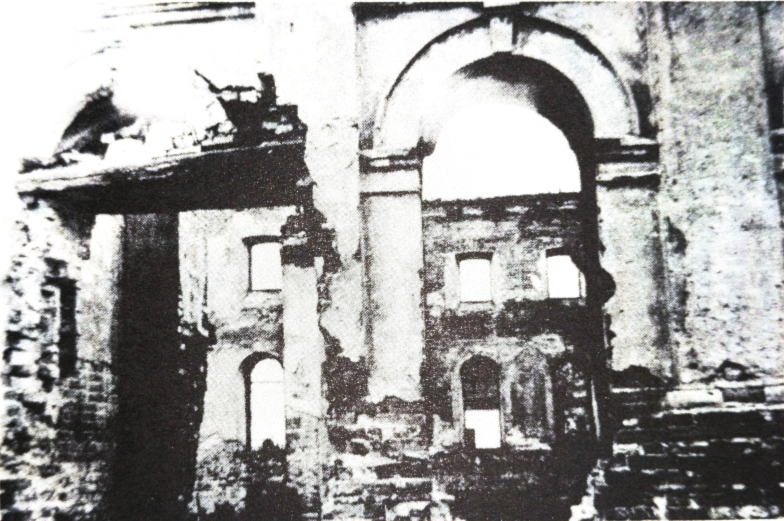
\includegraphics[width=7in]{Images/Saint_Mary_Church.png}}% Image to be included}
  \rotatebox{90}{% Rotate 90 CCW
    \begin{minipage}{\wd\stmary}
      \usebox{\stmary}
      \caption{Optina, the Church of St. Mary of Egypt --1978}
    \end{minipage}}
\end{figure}
\vspace*{\fill}\restoregeometry